\documentclass[notheorems]{beamer}
\usetheme{Madrid}
\usecolortheme{spruce}

\usepackage{graphicx} % Required for inserting images
\usepackage[romanian]{babel}
\usepackage[center]{caption}
\usepackage{float}
\usepackage{amsmath, amssymb}
\usepackage{mathtools}
\usepackage[T1]{fontenc}
\usepackage{ragged2e}

\usefonttheme[onlymath]{serif}

\theoremstyle{definition}
\newtheorem*{obs}{Observație}
\newtheorem{theorem}{Teoremă}
\newtheorem{proposition}{Propoziție}
\newtheorem{corollary}{Corolar}
\newtheorem{definition}{Definiție}
\newtheorem{lemma}{Lemă}

\AtBeginSection[]{
  \begin{frame}
  \vfill
  \centering
  \begin{beamercolorbox}[sep=8pt,center,shadow=true,rounded=true]{title}
    \usebeamerfont{title}\insertsectionhead\par%
  \end{beamercolorbox}
  \vfill
  \end{frame}
}

\newcommand{\E}{\mathbb{E}}

% \setbeamertemplate{items}[triangle]

\title[OrientInvest]{OrientInvest}
\author[Ș.P, A.T., G.T., A.T-B.]{
    Ștefan Patrichi \texttt{\small<stefan.patrichi.07@cnmbct.ro>}
    \texorpdfstring{\\}{}
    Andrei-Rareș Tănăsescu \texttt{\small<andrei.tanasescu@cnmbct.ro>}
    \texorpdfstring{\\}{}
    George-Mihai Tega \texttt{\small<george.tega@cnmbct.ro>}
    \texorpdfstring{\\}{}
    Alexandru Thury-Burileanu \texttt{\small<alexandru.thury-burileanu@cnmbct.ro>}
}

\institute[CNMB CT]{
    \normalsize
    Colegiul Național „Mircea cel Bătrân” Constanța
}

\date[ESTIC 2025]{Concursului pentru Elevi și Studenți în Tehnologia Informației\\24 mai 2025}

\begin{document}
\justifying
\frame{\titlepage}

\begin{frame}
\frametitle{Motivație, inspirație}
\begin{itemize}
    \item<2-> Pasiune pentru domeniul finanțelor
    \item<3-> Lansarea unui nou ETF pe energie la BVB (PTENGETF.RO)
    \item<4-> Dorința de a implementa instrumente de Deep Learning în optimizarea portofoliului (spre deosebire de cele tradiționale)
    \begin{itemize}
        \item<5-> \textit{Deep Learning for Portfolio Optimisation}, Zihao Zhang, Stefan Zohren, Stephen Roberts 
        (Oxford-Man Institute of Quantitative Finance,
        University of Oxford, 29 mai 2020)
    \end{itemize}
\end{itemize}
\end{frame}

\section{Despre ETF-uri}
\begin{frame} 
\frametitle{Ce este un ETF?}
\begin{itemize}
    \item<2-> \textit{Exchange-traded fund}
    \item<3-> Fond de investiții listat și tranzacționat pe piețele bursiere
    \item<4-> Adesea urmăresc un indice bursier
    \item<5-> iShares Core S\&P 500 ETF (IVV)
\end{itemize}
\end{frame}

\begin{frame}
\frametitle{Avantaje ale ETF-urilor}
\begin{itemize}
    \item<2-> Diversitate $\rightarrow$ Risc scăzut
    \item<3-> Administrare pasivă, costuri administrative mici $\rightarrow$ Rată a cheltuielilor mică
    \item<4-> Lichiditate, eficiență
\end{itemize}
\end{frame}

\section{Cum funcționează aplicația?}
\begin{frame}
\frametitle{Preluarea datelor}
\begin{itemize}
    \item<2-> Yahoo Finance (API -- biblioteca \texttt{yfinance})
    \item<3-> Adaptare la diferite calendare bursiere prin interpolare (biblioteca \texttt{pandas})
    \item<4-> Trecere la euro 
\end{itemize}
\end{frame}

\begin{frame}
    \frametitle{Măsurarea performanței unui portofoliu}
\begin{itemize}
    \item<2->$p(i, t) = $ prețul de închidere al activului $i$ la timpul (ziua) $t$.
    \item<3->Rata rentabilității: $\displaystyle r(i, t) = \frac{p(i, t) - p(i, t-1)}{p(i, t-1)} = \frac{p(i, t)}{p(i, t-1)} - 1$.
    \item<4->Ponderi (weights): $w(i, t) \in [0, 1]$ și $\displaystyle \sum_i w(i,t) = 1$ (prezise de rețeaua neuronală).
    \item<5->Portofoliul realizat: $\displaystyle R(t) = \sum_i w(i,t)\cdot r(i,t)$.
\end{itemize}
\end{frame}

\begin{frame}
\frametitle{Raportul Sharpe}
\begin{figure}
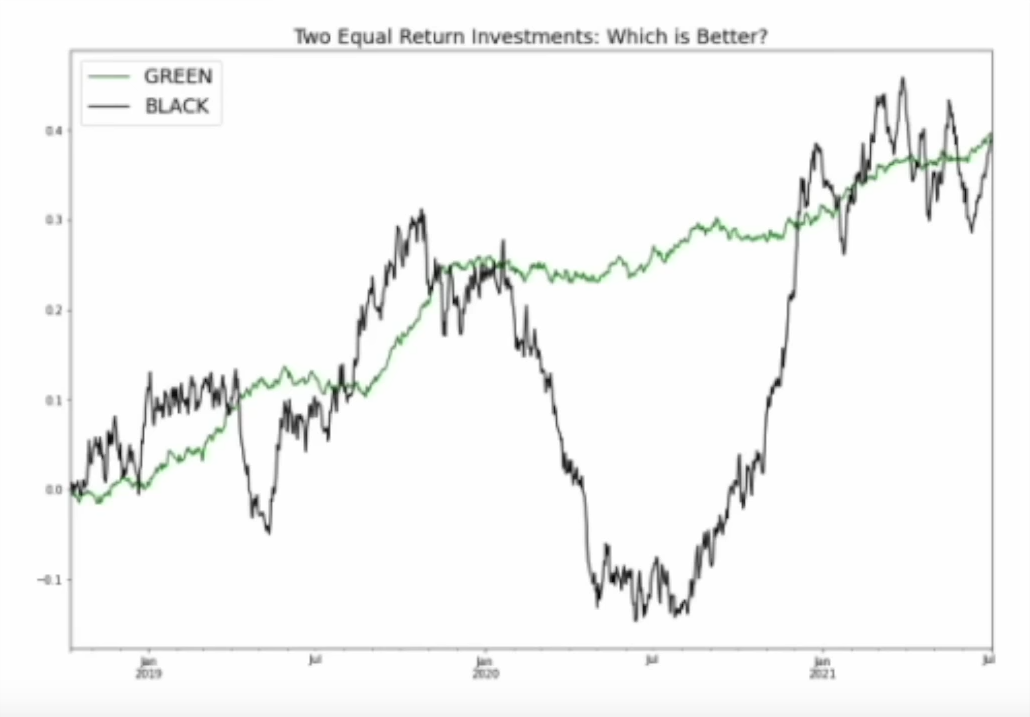
\includegraphics[scale=0.18]{images/sharpe.png}
\end{figure}
\begin{itemize}
    \item<2-> raportează performanța netă a portofoliului la riscul asumat \\($\approx$ abaterea standard)
    \only<3>{\item $\displaystyle L = \frac{\E[R(t)]}{\sigma} = \frac{\E[R(t)]}{\sqrt{\E[R^2(t)] - \E[R(t)]^2}}$}
    \only<4>{\item $\displaystyle L = \frac{\E[R(t)]}{\sigma} = \frac{\E[R(t)]}{\sqrt{\E[R^2(t)] - \E[R(t)]^2}} \cdot \sqrt{252}$}
\end{itemize}
\end{frame}

\begin{frame}
\frametitle{Softmax}
\begin{itemize}
    \item<1-> Modelul returnează ponderile care maximizează raportul Sharpe ($L$).
    \item<2-> Nu satisfac neapărat $w(i, t) \ge 0$ și $\displaystyle \sum_i w(i,t) = 1$!
    \item<3-> $\displaystyle \operatorname{softmax}(w(i, t)) = \frac{e^{w(i, t)}}{\sum\limits_{j=1}^n e^{w(j, t)}}$.
\end{itemize}
\end{frame}

\begin{frame}
\frametitle{Rețeaua neuronală}
\begin{itemize}
    \item<2-> 3 straturi:
    \begin{itemize}
        \item<3-> LSTM (32 neuroni, dropout: 0,2)
        \item<4-> Flatten
        \item<5-> Dense (Softmax)
    \end{itemize}
    \item<6-> Window-uri de câte 200 zile
    \item<7-> 80\% train, 20\% test
\end{itemize}
\end{frame}

\begin{frame}
\frametitle{Comunicare frontend -- backend}
\begin{itemize}
    \item<1-> API scris în biblioteca \texttt{fastapi}
    \item<2-> \texttt{index.html/process}
    \item<3-> \texttt{index.html/get\_etfs}
    \item<4-> \texttt{index.html/get\_etf\_history?etf=EPOL}
\end{itemize}
\end{frame}

\begin{frame}
\frametitle{Pagina web}
\begin{itemize}
    \item Grafice interactive în \texttt{plotly}
\end{itemize}
\end{frame}

\section{Limitări, posibilități de dezvoltare}
\begin{frame}
\frametitle{Limitări, posibilități de dezvoltare}
\begin{itemize}
    \item<1-> Anualizarea raportului Sharpe
    \item<2-> Mai multe ETF-uri listate la aceeași bursă
    \item<3-> Dezvoltare UI (ex. dropdown)
    \item<4-> Formulă alternativă pentru portofoliul realizat (volatilitate!) \\
    $\displaystyle R(t) = \sum_i \frac{\sigma_{tgt}}{\sigma(i,t-1)}w(i,t-1)\cdot r(i,t) 
    - C \cdot\sum_i\left|\frac{\sigma_{tgt}}{\sigma(i,t-1)}w(i,t-1) - \frac{\sigma_{tgt}}{\sigma(i,t-2)}w(i,t-2)\right|$
\end{itemize}
\end{frame}

\section{Vă mulțumim!}
\end{document}
